\section{Robotic Manipulator}
\label{Chapter:RoboticManipulator}
{
    \subsection{Functional Requirements of the Manipulator}
    {
        To fully test the twisting splines with a robot, a simple simulator was written as a desktop application. The following sections will now discuss a manipulator with six degrees of freedom used to test the splines. The details about working and design of the simulator are discussed in section \label{Chapter:Drogon} in Appendix 1. We now take a little diversion from the twisting splines to discuss the manipulator and then discuss their incorporation in the simulator in section \ref{Section:SimulatingRBS}.
    }
    \subsection{Functional Requirements of the Manipulator}
    {
        Typically, a robot is required to perform precise maneuvers with complete $6$ degrees of freedom of the end effector in both planar and curved planes. It is also required to provide at least one extra actuator to reduce singularities. In addition to position, the robot is also required to perform precise velocity and force controlled maneuvers. However, to use the test case of twisting bezier spline curves, not all of these functional requirements are forced. The manipulator has only six degrees of freedom and incorporates only a position control mechanism.
    }
    \subsection{Manipulator Representation}
    {
        Conventionally, the robot can be represented on a piece of paper using simple symbols and links as shown in Fig. \ref{FigConventionalRep}
        \begin{figure}[hb]
          \centering
          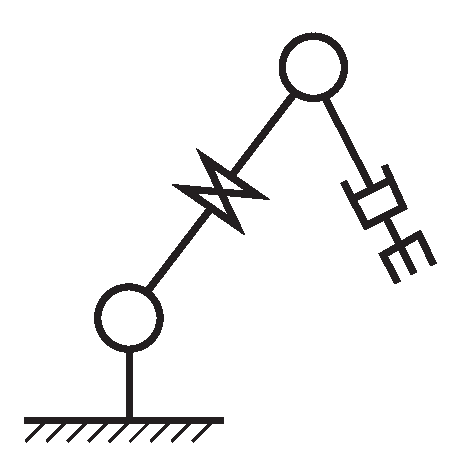
\includegraphics[width=0.5\textwidth]{../Images/RobotRep1.pdf}
          \caption{Conventional way of representing a manipulator. The circles show a rotation between the interconnected links on the plane of the paper. The cross symbol shows rotation on the link line. The square symbol is for prismatic joint. It represents change in length along the link line.}\label{FigConventionalRep}
        \end{figure}
        This kind of representation is clean and simple but doesn't give a complete view of the robot. Specially, with virtually zero link lengths, the visual representation can confuse someone new to the realm of robotic. Based on repeated experiments and to answer the weakness of contentional representation, we propose a new kind of representation that encapsulates the basic idea of representation with some features of a $D-H$ table. See Fig. \ref{FigMyRep}
        \begin{figure}
          \centering
          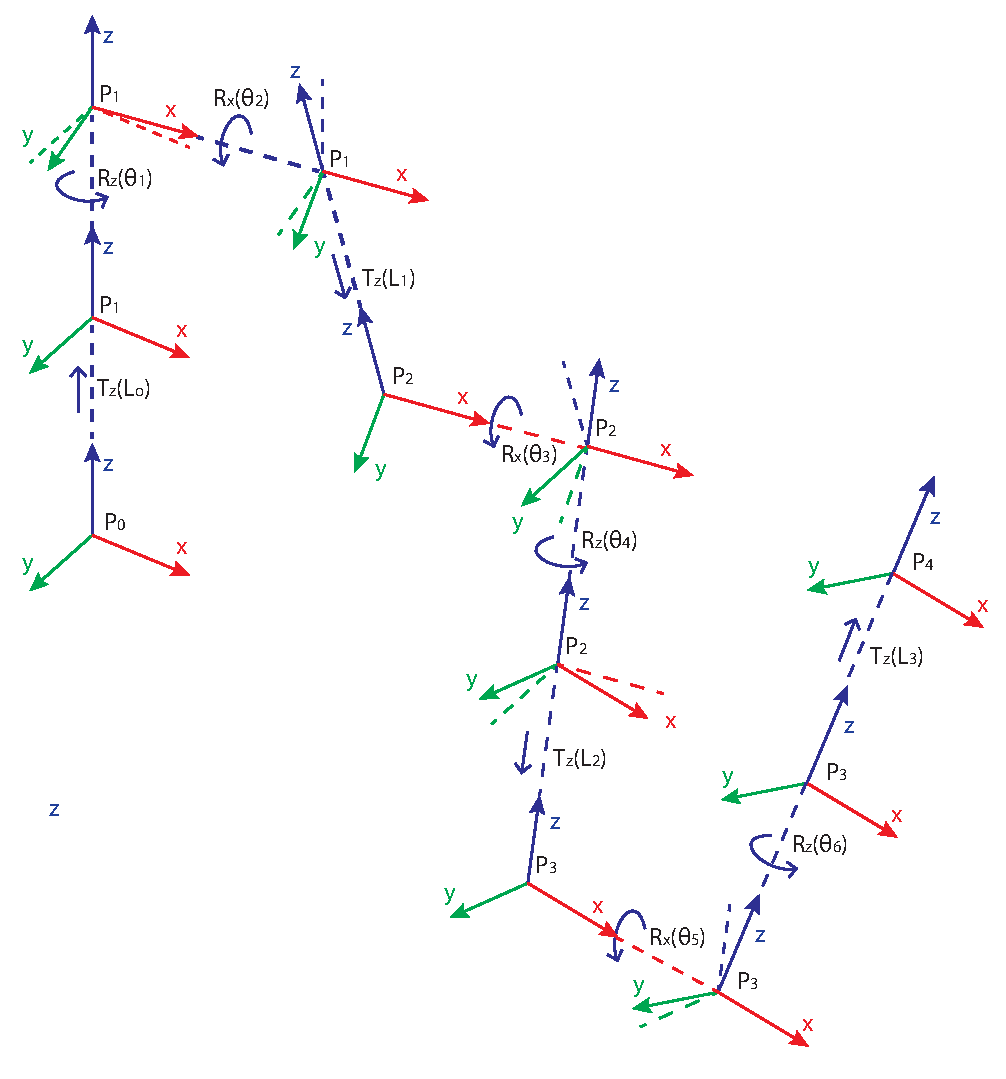
\includegraphics[width=0.8\textwidth]{../Images/MyRep.pdf}
          \caption{An example of \texttt{transformation frames} representation. This representation shows how a reference frame is linked to the previous using two basic transformation functions, $T_n$ and $R_n$ where n is the axis along or about which the transformation is performed. The schematic is drawn in the direction of $F0$ to $F_N$ ($N$ being the last frame) but can also be interpreted in reverse direction. One can easily see which transformations are required to convert one frame of reference to the other. One only needs to take one thing in account. When going in forward direction, all the transformations are applied as they are but while going back, each successive transformation is taken as inverse. For example, frame $F5$ can be achieved from frame $F3$ by applying two successive transformations: translation along $x$ of magnitude $L1$ and rotation about $x$ of magnitude $\theta_3$. However, to go to frame $F3$ from frame $F5$, one needs to apply two successive transformations: rotation about $x$ of magnitude $-\theta_3$ and translation along \texttt{x} of magnitude $-L1$. It should be noted that if a transformation changes the origin of the frame, the next frame has a different point shown at the center. This point is defined in the base frame.
          } \label{FigMyRep}
        \end{figure}

        Interestingly, this representation can't only represent physical manipulators, it can also represent abstract transformations. See Fig. \ref{FigEulerRep} which represents a target $P_t$ being represented as $z-x-z$ euler angles.

        \begin{figure}
          \centering
          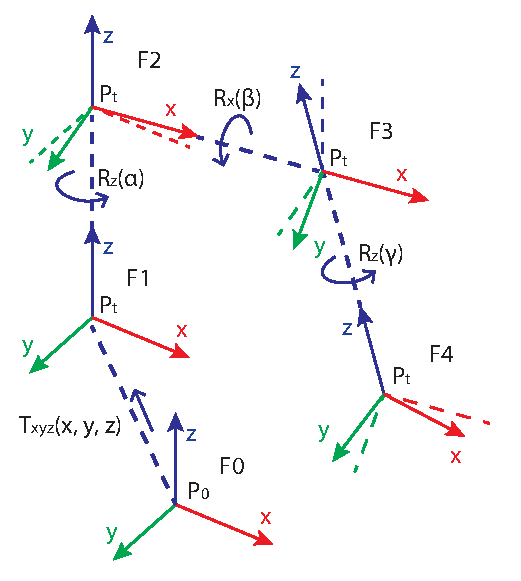
\includegraphics[width=0.6\textwidth]{../Images/EulerANgles.pdf}
          \caption{Three successive rotation $z-x-z$ and similar orders are call \texttt{Euler Angles Transformations}. A base Frame $F0$ is transformed though three translations and three euler rotations. This way, one can easily represent a target point to the robot which would have three extra components than $x$, $y$ and $z$; $\alpha$, $\beta$a and $\gamma$.
          } \label{FigEulerRep}
        \end{figure}

        Now, if one represents both target and the manipulator representation in a solved state, a closed loop representation can be formed which becomes extremely convenient in inverse kinematics. See Fig. \ref{FigCompleteRep} which exemplifies a closed loop \texttt{transformation frames} representation. It should be quite clear that once a closed loop is constructed, one can make transformations in any direction.

        \begin{figure}
          \centering
          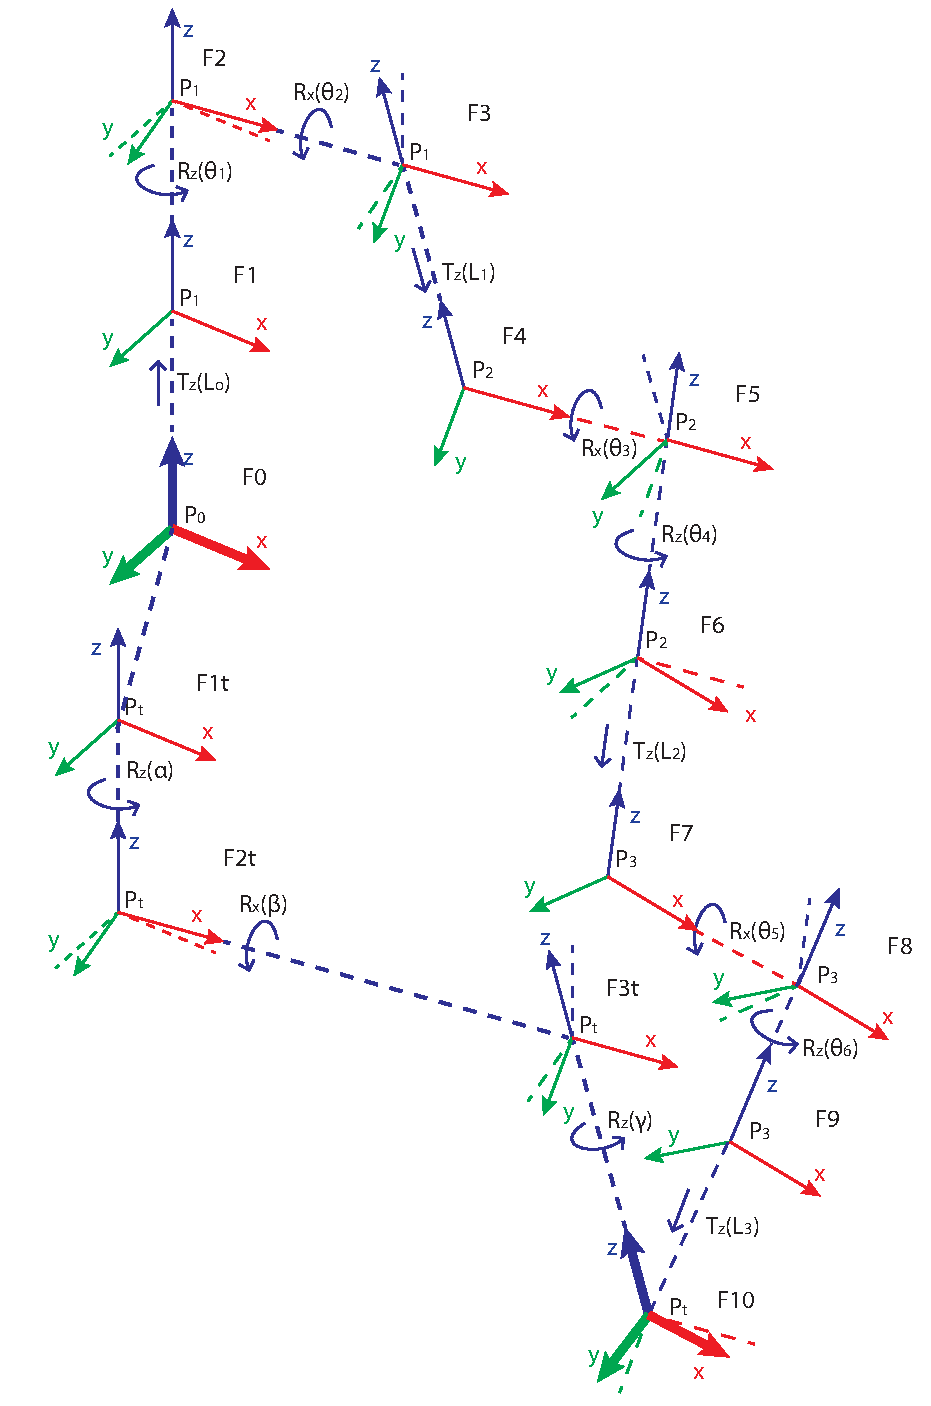
\includegraphics[width=0.8\textwidth]{../Images/CompleteRep.pdf}
          \caption{A manipulator along with a target represented in \texttt{transformation frames} representation. $F0$ corresponds to the base frame, $F0, F1, F2 ...$ represent the forward direction of the manipulator and $Ft0, Ft1, Ft2 ...$ represent the forward direction of the target. Both chains of transformations lead to a common reference frame eventually, the target frame of reference, or the end-effector frame of reference, $Ft$.
          } \label{FigCompleteRep}
        \end{figure}

        It is interesting to see that while doing a complete cycle transformation, one virtually transforms a frame through nothing! Also, if a $N-1$ frame transformation is applied in a $N$ frame closed loop, one can identify one last transformation quite easily by comparing the initial and the final frames. This method is called \texttt{Known Error Propagation} and will be used extensively in the inverse kinematics.

        Last, but not the least, of the usages of a closed loop representation is that some transformations can be skipped/swapped safely in order to simplify the loop. This can lead to finding further more unknown parameters using \texttt{Known Error Propagation}.

    }
    \subsection{Selecting a Configuration}
    {
        The configuration selected for this project is widely used by other engineers but the main inspiration behind choosing this configuration was a B.Sc. final year project of the \emph{Mechanical Engineering Department of U.E.T} of the batch $12$' with title, 'Design and Implementation of a $6$DoF Spot Welding Robot'. The project report presents a solution and describes all the forward and inverse kinematics. And all this, without using a regular transformation matrix! The effort in the current project takes some inspiration from the previous one and also elaborates not only the faults and issues with the previous but also the effectiveness of using transformation matrices.

        See Fig. \ref{FigCompleteRep} which represents this manipulator. It has six rotating actuators linked together with four links.
    }
    \subsection{Mathematical Modelling}
    {
        Using the new representation, properties of homogenous transformation matrices and basic highschool trigonometry, I was able to calculate \cite{bib21} the unique and redundant solutions for the spherical manipulator. The manipulator has two primary solutions: different joint positions yield the same end effector position and orientation. Connected to both solutions, are $4$ more secondary solutions which effect only the motor angles not the link locations.

        Finding out the mathematical equations is one job, verification is another. While dealing with three dimensional realm on a two dimensional paper, one can the solution but making small human errors on the way. It is quite easy to confuse the directions of rotations in a reference frames, resulting in typical errors which can be mitigated by some hit-and-trial of a few operations; adding or subtracting integral multiples of $\frac{\pi}{2}$ from the angles, inverting the length signs, inverting the angle directions. This can be done easily only if a representation tool is build alongside the robot modeling.
    }

    \subsection{Inverse and Forward Kinematics}
    {
        Some of the motor angles are quite obvious. See the series of hand-sketched figures labelled with mask Fig. \texttt{RDn} in the subsequent pages which demonstrate how an inverse kinematic solution was discovered for this robot.
    }

    \subsection{Incorporating the twisting bezier splines} \label{Section:SimulatingRBS}
    {
        Using the same model of the spline model, the simulator first rasterizes the whole spline and then transforms the two dimensional points onto a plannar surface simulated on a user desired position in the workspace. Then it creates a pseudo machine code to mimic the tool changes required before each stroke and the transformed rasterized points are directly considered as G-Codes for the manipulator. Once computed it starts implementing the program.

        For the sake of analysis, in parallel, the end effector orientation is captured continuously to construct an ink mark with each sweep of the tool. The reproduced image is then used for analysis. The results of such a comparison can be seen in Table \ref{Table:MachineDataMetrices}. The value indicate that the robot very closely reproduces the given spline thus verifying the thesis of the research.

        \begin{table}[ht]
        \centering
        \resizebox{\textwidth}{!}{\begin{tabular}{| p{0.3\linewidth} | p{0.3\linewidth} |  p{0.2\linewidth} |  p{0.2\linewidth} |}
          \hline
          & \textbf{Reference} & \textbf{Coverage} & \textbf{Extra} \\
          \hline
          \multicolumn{4}{|l|}{\textbf{Nastaleeq}}\\
          \hline
          Rotating Bazier Spline & Original Image & 95.8\% & 5.4\% \\
          \hline
          Machined Output & Original Image & 96.7\% & 7.0\% \\
          \hline
          Machined Output & Rasterized Image & 96.7\% & 4.3\% \\
          \hline
          \multicolumn{4}{|l|}{\textbf{Thuluth}}\\
          \hline
          Rotating Bazier Spline & Original Image & 93.4\% & 2.8\% \\
          \hline
          Machined Output & Original Image & 95.0\% & 3.4\% \\
          \hline
          Machined Output & Rasterized Image & 97.8\% & 4.4\% \\
          \hline
        \end{tabular}}
        \caption{Benchmark of the mathematical accuracy of the twisting bezier spline curves with a simulated manipulator}
        \label{Table:MachineDataMetrices}
        \end{table}
    }
}
\clearpage 